\documentclass[12pt]{article}

\usepackage[margin=1in]{geometry}
\usepackage[T1]{fontenc}
\usepackage[utf8]{inputenc}
\usepackage{amsmath,amssymb}
\usepackage{booktabs}
\usepackage{multirow}
\usepackage{graphicx}
\usepackage{subcaption}
\usepackage{float}
\usepackage{setspace}
\usepackage{lineno}
\usepackage[authoryear,round]{natbib}
\usepackage{hyperref}

\onehalfspacing
% \linenumbers   % uncomment if the prof wants line numbers for review

\title{EcoExplain-VLM: Evaluating Vision--Language Models for Forest Disturbance
Classification from Multi-Source Satellite Evidence in Kanha Tiger Reserve}
\author{Your Name \\ Your Department, Institute}
\date{}

\begin{document}
\maketitle

\begin{abstract}
% ~250 words: problem, data, method, key numbers, takeaway
\end{abstract}

\noindent\textbf{Keywords:} forest disturbance; vision--language models; Sentinel-2;
Sentinel-1 SAR; change detection; Kanha Tiger Reserve

%======================================================================
\section{Introduction}
% 1000--1200 words. Focus -> motivation/rationale -> gap -> objectives.
% Keep it as continuous prose; objectives can be a short numbered list at the end.

%======================================================================
\section{Data and Methodology}

\subsection{Study Area}
% Kanha Tiger Reserve, Madhya Pradesh. Full India map with no trimming at the top.
\begin{figure}[H]
  \centering
  % \includegraphics[width=\textwidth]{figures/study_area.png}
  \caption{(a) Location of Kanha Tiger Reserve in India; (b) reserve boundary with patch grid.}
  \label{fig:study_area}
\end{figure}

\subsection{Data}
\subsubsection{Optical and SAR Imagery}
% Sentinel-2 (T0: Jan--Feb 2022, T1: Jan--Feb 2023), Sentinel-1 VV/VH

\subsubsection{Ancillary Data}
% CHIRPS, ERA5-Land, NASADEM

\begin{table}[H]
  \centering
  \caption{Datasets used in this study.}
  \label{tab:data}
  \begin{tabular}{llll}
    \toprule
    Dataset & Variables & Resolution & Source \\
    \midrule
     &  &  &  \\
    \bottomrule
  \end{tabular}
\end{table}

\subsection{Preprocessing and Patch Generation}
% GEE export, compositing, cloud masking, 512x512 patches, T0/T1 RGB

\subsection{Disturbance Evidence and Labelling}
% Spectral indices, differencing, Otsu thresholding, evidence text, stable/decline/increase labels
\begin{equation}
  \mathrm{NDVI} = \frac{\rho_{\mathrm{NIR}} - \rho_{\mathrm{Red}}}{\rho_{\mathrm{NIR}} + \rho_{\mathrm{Red}}}
  \label{eq:ndvi}
\end{equation}

\subsection{Dataset Construction and Splits}
% 366 patches, dataset.jsonl, stratified 70/15/15 split (seed 42): 256/55/55

\subsection{Vision--Language Models and Evaluation}
\subsubsection{Zero-shot Benchmark}
% LLaVA-1.5, PaliGemma, Qwen2-VL, BLIP-2; same prompt (Condition C)

\subsubsection{Fine-tuning}
% LoRA on Qwen2-VL-2B, train split only; hyperparameters in a table or appendix

\subsubsection{Evaluation Metrics}
\begin{equation}
  \mathrm{Accuracy} = \frac{1}{N}\sum_{i=1}^{N} \mathbb{1}\left(\hat{y}_i = y_i\right)
  \label{eq:acc}
\end{equation}

\begin{figure}[H]
  \centering
  % 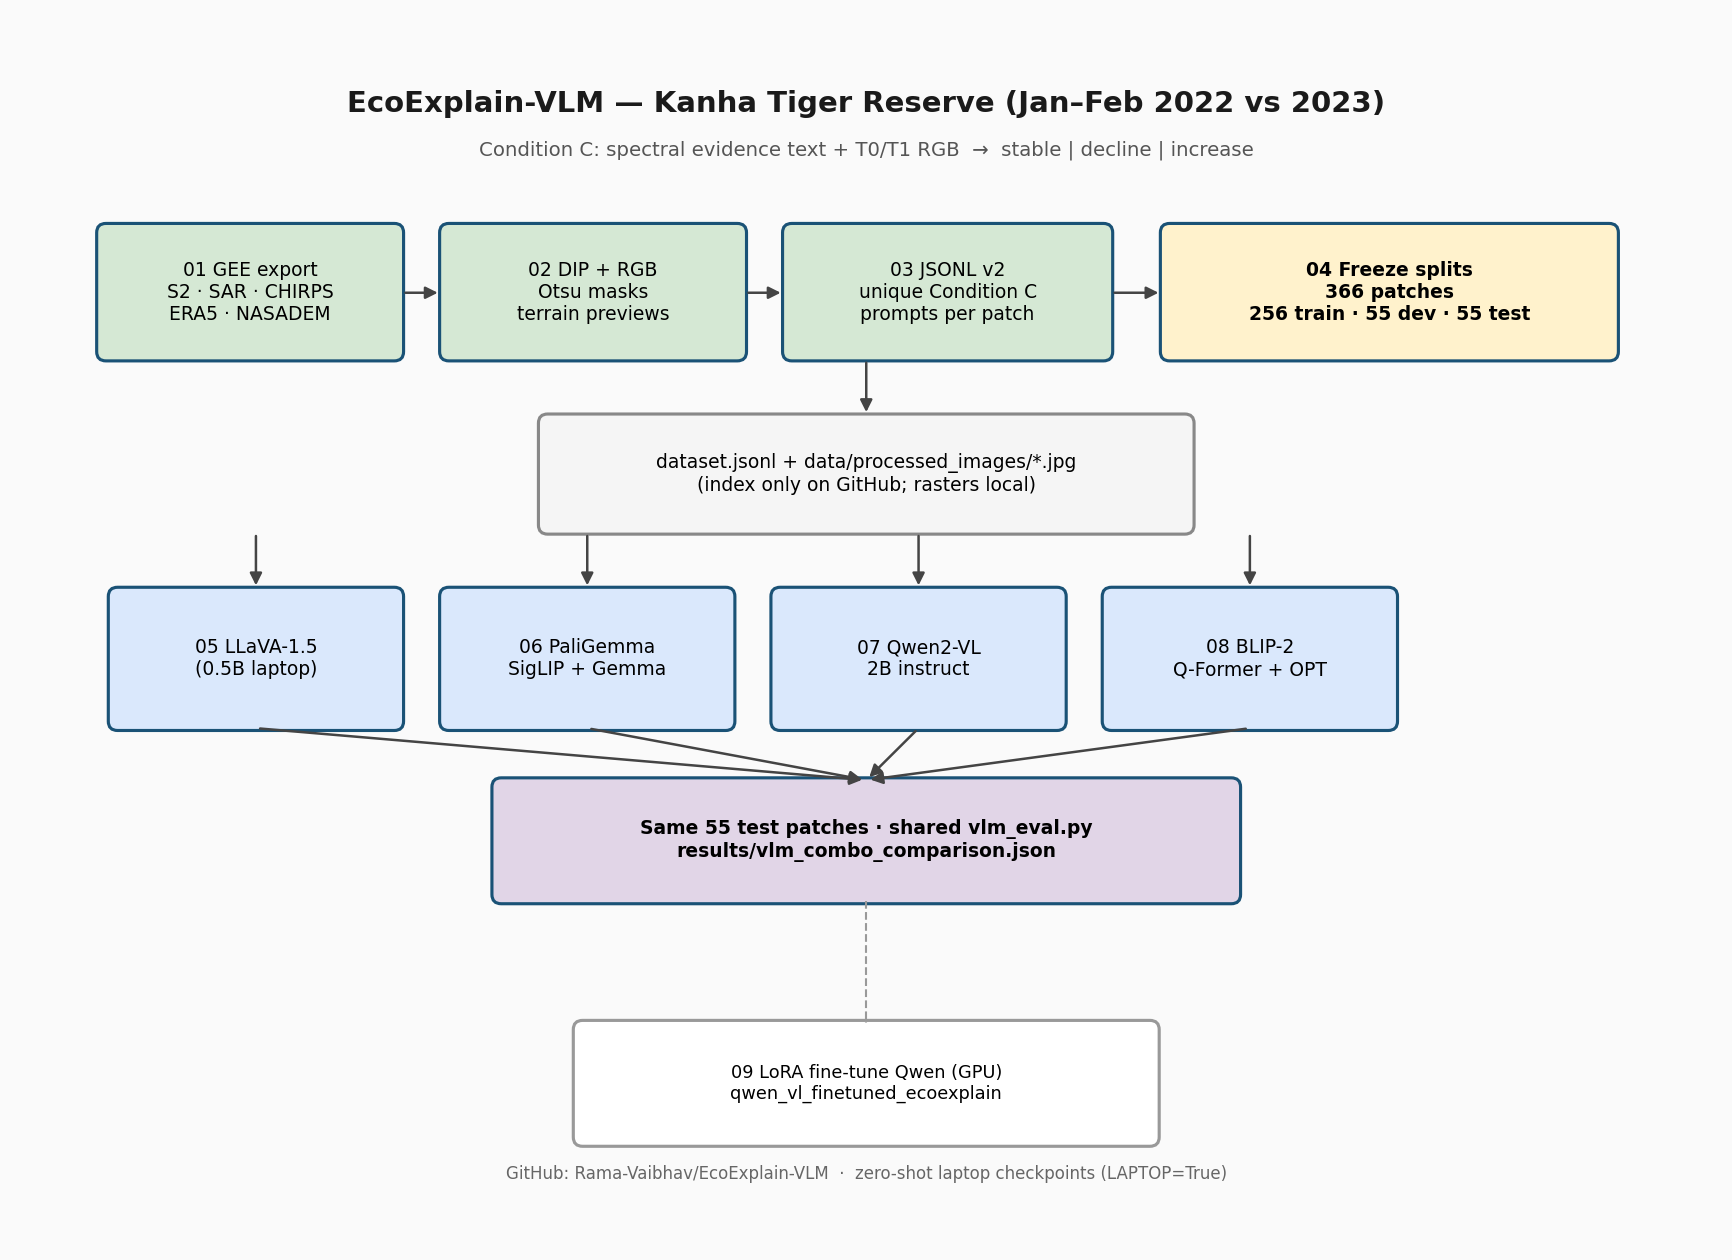
\includegraphics[width=\textwidth]{results/result1.png}
  \caption{Overall workflow of the study.}
  \label{fig:workflow}
\end{figure}

%======================================================================
\section{Results and Discussion}

\subsection{Dataset Characteristics}
% Class distribution, pilot agreement (auto vs human), example patches

\subsection{Zero-shot Model Performance}
\begin{table}[H]
  \centering
  \caption{Zero-shot accuracy on the test split ($n=55$).}
  \label{tab:zeroshot}
  \begin{tabular}{clc}
    \toprule
    Rank & Model & Accuracy (\%) \\
    \midrule
     &  &  \\
    \bottomrule
  \end{tabular}
\end{table}

\subsection{Effect of Fine-tuning}

\subsection{Error Analysis}
% Confusion matrices, sample failures; combine as Fig. (a), (b), (c)
\begin{figure}[H]
  \centering
  \begin{subfigure}{0.48\textwidth}
    % \includegraphics[width=\linewidth]{figures/cm_zeroshot.png}
    \caption{}
  \end{subfigure}
  \hfill
  \begin{subfigure}{0.48\textwidth}
    % \includegraphics[width=\linewidth]{figures/cm_finetuned.png}
    \caption{}
  \end{subfigure}
  \caption{(a) Zero-shot and (b) fine-tuned confusion matrices.}
  \label{fig:confusion}
\end{figure}

\subsection{Comparison with Previous Studies}

%======================================================================
\section{Limitations and Future Scope}

%======================================================================
\section{Conclusions}

%======================================================================
\section*{Acknowledgements}
% Copernicus/ESA (Sentinel-1/2), CHG/UCSB (CHIRPS), ECMWF (ERA5-Land),
% NASA (NASADEM), Google Earth Engine, Hugging Face, IIIT Ada HPC, supervisor

%======================================================================
\bibliographystyle{apalike}
\bibliography{references}   % create references.bib; cite only what you use

%======================================================================
\clearpage
\appendix
\renewcommand{\thetable}{A\arabic{table}}
\renewcommand{\thefigure}{A\arabic{figure}}
\setcounter{table}{0}
\setcounter{figure}{0}
\section*{Appendix}
% Appendix Table A1: LoRA hyperparameters
% Appendix Table A2: per-model prompt / parsing details
% Appendix Figure A1: example T0/T1 patches per class

\end{document}
